\documentclass{article}

\usepackage{fancyhdr}
\usepackage{extramarks}
\usepackage{amsmath}
\usepackage{amsthm}
\usepackage{amsfonts}
\usepackage{tikz}
\usepackage[plain]{algorithm}
%\usepackage{algpseudocode}
\usepackage{amssymb}
\usepackage{enumitem}
\usepackage{relsize}
\usepackage{textcomp}
\usepackage{graphicx}
\usepackage{bm}
%\usepackage{textcomp}
%\usepackage{tabularx}
\usepackage{xcolor,colortbl}

%\usetikzlibrary{automata,positioning}
%\usepgfplotslibrary{external} 
%\tikzexternalize

%
% Basic Document Settings
%

\topmargin=-0.45in
\evensidemargin=0in
\oddsidemargin=0in
\textwidth=6.5in
\textheight=9.0in
\headsep=0.25in

\linespread{1.1}

\pagestyle{fancy}
\lhead{\hmwkAuthorName}
\chead{\hmwkClass\ (\hmwkClassInstructor\ \hmwkClassTime): \hmwkTitle}
\rhead{\hmwkDueDate}
\lfoot{\lastxmark}
\cfoot{\thepage}

\newcommand{\minus}{\scalebox{0.5}[1.0]{$-$}}
\newcommand\tab[1][0.5cm]{\hspace*{#1}}
\renewcommand\headrulewidth{0.4pt}
\renewcommand\footrulewidth{0.4pt}
\renewcommand{\theenumi}{\Alph{enumi}}

\setlength\parindent{0pt}

%
% Create Problem Sections
%

\newcommand{\enterProblemHeader}[1]{
	\nobreak\extramarks{}{{#1} continued on next page\ldots}\nobreak{}
	\nobreak\extramarks{{#1} (continued)}{{#1} continued on next page\ldots}\nobreak{}
}

\newcommand{\exitProblemHeader}[1]{
	\nobreak\extramarks{{#1} (continued)}{{#1} continued on next page\ldots}\nobreak{}
	\stepcounter{homeworkProblemCounter}
	\nobreak\extramarks{{#1}}{}\nobreak{}
}

\newcounter{homeworkProblemCounter}
\setcounter{secnumdepth}{0}
\newcounter{partCounter}
\nobreak\extramarks{Problem \arabic{homeworkProblemCounter}}{}\nobreak{}

\newenvironment{homeworkProblem}[1][-1]{
	\subsection*{{#1}:}
	\enterProblemHeader{{#1}}
	\exitProblemHeader{{#1}}
}

\newcommand{\hmwkTitle}{Chapter 8 Homework}
\newcommand{\hmwkDueDate}{October 4, 2019}
\newcommand{\hmwkClass}{MTH 5051}
\newcommand{\hmwkClassTime}{Section 01}
\newcommand{\hmwkClassInstructor}{Dr. Jim Jones}
\newcommand{\hmwkAuthorName}{\textbf{Eric Pereira}}

%
% Title Page
%
\pagenumbering{gobble}
\title{
	\vspace{2in}
	\textmd{\textbf{\hmwkClass:\ \hmwkTitle}}\\
	\normalsize\vspace{0.1in}\small{Due\ on\ \hmwkDueDate\ at 11:59pm}\\
	\vspace{0.1in}\large{\textit{\hmwkClassInstructor\ \hmwkClassTime}}
	\vspace{3in}
}

\author{\hmwkAuthorName}
\date{}

\renewcommand{\part}[1]{\textbf{\large Part \Alph{partCounter}}\stepcounter{partCounter}\\}

%
% Various Helper Commands
%

% Useful for algorithms
\newcommand{\alg}[1]{\textsc{\bfseries \footnotesize #1}}

% For derivatives
\newcommand{\deriv}[1]{\frac{\mathrm{d}}{\mathrm{d}x} (#1)}

% For partial derivatives
\newcommand{\pderiv}[2]{\frac{\partial}{\partial #1} (#2)}

% Integral dx
\newcommand{\dx}{\mathrm{d}x}

% Alias for the Solution section header
\newcommand{\solution}{\textbf{\large Solution}}

% Probability commands: Expectation, Variance, Covariance, Bias
\newcommand{\E}{\mathrm{E}}
\newcommand{\Var}{\mathrm{Var}}
\newcommand{\Cov}{\mathrm{Cov}}
\newcommand{\Bias}{\mathrm{Bias}}

\begin{document}
	\maketitle
	
	\pagebreak
	\pagenumbering{arabic}
	
	
	%%%%%%%%%%%%%%%%%%%      
	%	NEW SECTION   %
	%%%%%%%%%%%%%%%%%%%
	\section{Chapter 8.1}
	
	%%%%%%%%%%%%%%%%%%%%%%%%%%%%%%%%%%%%%%%%%%%%%%%%%%%%%%%%%%%%%%%%%%%%%%%%%%%%%%%%%%
	%                                                                                %
	%                          Section 8.1 Problem 5                                 %
	%                                                                                %
	%%%%%%%%%%%%%%%%%%%%%%%%%%%%%%%%%%%%%%%%%%%%%%%%%%%%%%%%%%%%%%%%%%%%%%%%%%%%%%%%%%
	
	\begin{homeworkProblem}[Problem 5]
		\tab Determine the number of positive integers $n$, $1\le n \le 2000$, that are
		\begin{enumerate}[label=(\alph*)]
			\item Not divisible by 2, 3, or 5
			\item Not divisible by 2, 3, 5, or 7
			\item Not divisible by 2, 3, or 5, but are divisible by 7.
		\end{enumerate}
		
		
		\textbf{\\Solution:}
		\begin{enumerate}[label=(\alph*)]
			\item The way to do this is to subtract each divisble amount out of 2000, and 
				add the values that 2,3, and 5 have in common as we double counted those. 
				After that you have to subtract the values that all 3 share as we double 
				counted those. By the laws of inclusion and exclusion you add all the 
				even numbers and subtract all the odd number cases, so thats exactly what
				happnes. Because this is a problem of inclusion and exclusion
				we can denote 2 as $c_1$, 3 as $c_2$ and 5 as $c_3$ We can do this by:
				\begin{align*}
					&N(c_1)=2000/2=1000,\ N(c_2)2000/3=666,\ N(c_3)2000/5=400 \\
					&N(c_1c_2)=2000/(2*3)=333,\ N(c_1c_3)=2000/(2*5)=200,
					\ N(c_2c_3)=2000/(3*5)=133 \\
					&N(c_1c_2c_3)2000/(2*3*5)=66 \\
					&N(\bar{c_1}\bar{c_2}\bar{c_3})=2000-[N(c_1)+N(c_2)+N(c_3)]+
					[N(c_1c_2)+N(c_1c_3)+N(c_2c_3)]-N(c_1c_2c_3)=\bm{534}
				\end{align*}
			\item We do essentially the same as we did before, except because there are 
				4 values instead of 3 there are many more shared values that we have to 
				subtract. After this, we double subtracted the value that all 4 share, so
				we have to add those. We can now label 7 as $c_4$ This can be expressed in 
				our equations:
				\begin{align*}
					&N(c_1)=2000/c_1=1000,\ N(c_2)2000/c_2=666,\ N(c_3)2000/c_3=400,
					\ N(c_4)=2000/c_4=285 \\
					&N(c_1c_2)=2000/(c_1c_2)=333,\ N(c_1c_3)=2000/(c_1c_3)=200,\ N(c_2c_3)=2000/(c_2c_3)
					=133, \\
					&\qquad \qquad \qquad
					N(c_1c_4)=2000/(c_1c_4)=142, N(c_2c_4)2000/(c_2c_4)=95,\ N(c_3c_4)=2000/(c_3c_4)=57 \\
					&N(c_1c_2c_3)=2000/(c_1c_2c_3)=66,\ N(c_1c_2c_4)=2000/(c_1c_2c_4)=47,
					\ N(c_2c_3c_4)=2000/(c_2c_3c_4)=19, \\
					&\qquad \qquad \qquad \ N(c_1c_3c_4)=2000/(c_1c_3c_4)=28 \\
					&N(c_1c_2c_3c_4)=2000/(2\cdot 3\cdot 5\cdot 7)=9\\
					&N(\bar{c_1}\bar{c_2}\bar{c_3}\bar{c_4})=2000-(1000+666+400+285)+(333+200+133+142+95+57) \\
					& \qquad \qquad \qquad-(66+47+19+28)+9=\bm{458}
				\end{align*}
			\item In order to easily do this you can get all the values from (a) and subtract
				them in (b). This would be:
				\begin{align*}
					534-458=\bm{76}
				\end{align*}
		\end{enumerate}
		
	\end{homeworkProblem} 

	%%%%%%%%%%%%%%%%%%%%%%%%%%%%%%%%%%%%%%%%%%%%%%%%%%%%%%%%%%%%%%%%%%%%%%%%%%%%%%%%%%
	%                                                                                %
	%                          Section 8.1 Problem 7                                 %
	%                                                                                %
	%%%%%%%%%%%%%%%%%%%%%%%%%%%%%%%%%%%%%%%%%%%%%%%%%%%%%%%%%%%%%%%%%%%%%%%%%%%%%%%%%%
	
	\begin{homeworkProblem}[Problem 7]
		\tab In how many ways can one arrange all of the letters in the word INFORMATION so 
		that no pair of consecutive letters occurs more than once? [Here we want to count 
		arrangements such as IINNOOFRMTA and FORTMAIINON but not INFORINMOTA
		(where "IN" occurs twice) or NORTFNOIAMI (where "NO" occurs twice).]
		
		\textbf{\\Solution:}
		
		\tab First we have to find all the possible pairs that can occur more than once.
		The possible pairs are: 
		\begin{center}
			\{IN, NI, NO, ON, IO, OI\}
		\end{center}
		\tab This is due to have 3 repeating letters \{I, N, O\}. \\
		\tab Let's now start by finding the total possible arrangements. The total
		possible arrangements is the 11 letters but making sure we don't count the 
		repeat values. This would be counted by:
		\begin{align*}
			N=\frac{11!}{(2!)^3}
		\end{align*}
		\tab After this we need to find the criteria for single instances where IN, and 
		alike letter combos afforementioned appear and where the possible combos of certain
		letters appear. We can describe the array mentioned above by letters $c_1$-$c_6$ in
		that order. We can get these equations by:
		\begin{align*}
			&N(c_1)=9!/(2!)^2 \\
			&N(c_1)=N(c_2)=N(c_3)=N(c_4)=N(c_5)=N(c_6) \\
			&N(c_1c_2)=0 \text{ impossible to have pairs of IN and NI in one word} \\
			&N(c_1c_2)=N(c_1c_4)=N(c_1c_5)=N(c_2c_3)=N(c_2c_6) \\
			&\qquad \quad \ =N(c_3c_4)=N(c_3c_5)=N(c_4c_6)=N(c_5c_6) \\
			&N(c_1c_3)=\frac{7!}{2!} \\
			&N(c_1c_3)=N(c_1c_6)=N(c_2c_4)=N(c_2c_5)=N(c_3c_6)=N(c_4c_5) \\ \\
			&\text{because 3, 4, 5, and 6 pairs do not exist in this case, these are all 0} \\ \\
			&S_0=N=4,989,600 , \qquad S_1=N(c_1)\cdot6=544,320 , \qquad S_2=N(c_1c_3)\cdot6=15,120 \\
			&S_0-S_1+S_2=4,989,600-544,320+15,120=\bm{4,460,400}
		\end{align*}
		
		
	\end{homeworkProblem} 


	%%%%%%%%%%%%%%%%%%%%%%%%%%%%%%%%%%%%%%%%%%%%%%%%%%%%%%%%%%%%%%%%%%%%%%%%%%%%%%%%%%
	%                                                                                %
	%                          Section 8.1 Problem 11                                %
	%                                                                                %
	%%%%%%%%%%%%%%%%%%%%%%%%%%%%%%%%%%%%%%%%%%%%%%%%%%%%%%%%%%%%%%%%%%%%%%%%%%%%%%%%%%
	
	\begin{homeworkProblem}[Problem 11]
		\tab At Flo's Flower Shop, Flo wants to arrange 15 different plants on five shelves 
		for a window display.  In how many ways can she arrange them so that each shelf has 
		at least one, but no more than four, plants?
		
		\textbf{\\Solution:}
		
		Well, Initially, we have to understand that we have to place at least one of the plants
		on each window display, which gives us 10 ``free plants" (free as in they can go to 
		any other window display after that). However, we have to consider that there is a limit 
		of 4 plants per display. 
		
		
	\end{homeworkProblem} 

	%%%%%%%%%%%%%%%%%%%%%%%%%%%%%%%%%%%%%%%%%%%%%%%%%%%%%%%%%%%%%%%%%%%%%%%%%%%%%%%%%%
	%                                                                                %
	%                          Section 8.1 Problem 13                                %
	%                                                                                %
	%%%%%%%%%%%%%%%%%%%%%%%%%%%%%%%%%%%%%%%%%%%%%%%%%%%%%%%%%%%%%%%%%%%%%%%%%%%%%%%%%%
	
	\begin{homeworkProblem}[Problem 13]
		\tab Find the number of permutations of $a, b, c, ..., x, y, z,$ in
		which none of the patterns $spin$, $game$, $path$, or $net$ occurs.
		
		\textbf{Solution:}
		
		\tab In this case, we can start by figuring out $N$ which is pretty easy. It's 
		just 26! for each letter in the alphabet. Now we have to calculate each instance 
		of each work. Let's say $spin$ is $c_1$, $game$ is $c_2$, $path$ is $c_3$, and
		$net$ is $c_4$. $c_1$ is the same length as $c_2$ and $c_3$ are the same length
		they all are equal to each other. This can be explained by:
		\begin{align*}
			&N(c_1) = (26-4+1)! = 23! \\
			&N(c_1) = N(c_2) = N(c_3)
		\end{align*}
		\tab Because $c_4$ is 3 letters it is instead:
		\begin{align*}
			N(c_4)=(26-3+1)!=24!
		\end{align*}
		\tab Now, the only cases where 2 of the words can occur is with $spin$ and $net$
		and $spin$ and $game$ However, $spinet$ and some combo of $spin$ and $game$ use 
		different amounts of letters. This would look like.
		\begin{align*}
			&N(c_1c_2)=(26-8+2)!=20! \\
			&N(c_1c_4)=(26-6+1)!=21! \\
			&N(c_1c_3)=N(c_2c_3)=N(c_2c_4)=N(c_3c_4)=0 \\
			&N(c_1c_2c_3)=N(c_1c_2c_4)=N(c_1c_3c_4)=N(c_2c_3c_4)=0 \\
			&N(c_1c_2c_3c_4)=0
		\end{align*}
		\tab When doing final calculations they look like:
		\begin{align*}
			26!-(3(23!)+24!) + (20!+21!)
		\end{align*}
		
		
	\end{homeworkProblem} 

	%%%%%%%%%%%%%%%%%%%%%%%%%%%%%%%%%%%%%%%%%%%%%%%%%%%%%%%%%%%%%%%%%%%%%%%%%%%%%%%%%%
	%                                                                                %
	%                          Section 8.1 Problem 16                                %
	%                                                                                %
	%%%%%%%%%%%%%%%%%%%%%%%%%%%%%%%%%%%%%%%%%%%%%%%%%%%%%%%%%%%%%%%%%%%%%%%%%%%%%%%%%%
	
	\begin{homeworkProblem}[Problem 16]
		\tab How many social security numbers (nine-digit sequences)
		have each of the digits 1,3, and 7 appearing at least once?
		
		\textbf{\\Solution:}
		
		\tab a social security number consists of nine digits, so lets count every possible
		social security initially. This value would be:
		\begin{align*}
			10^9
		\end{align*}
		\tab Now by the laws of inclusion and exclusion we have to include the case scenarios
		where this value includes either the values of the 3 numbers 1,3,7. In order to do 
		this we have to calculate which numbers have either, 1, 2, or 3 of these values. When
		we subtract the values we have to consider that we will not have 10 numbers available but
		10 - num of digits appearing as we can only have 1,3, and 7 occur once. The 
		calculation would look like:
		\begin{align*}
			10^9-\binom{3}{1}9^9+\binom{3}{2}8^9-\binom{3}{3}7^9= \bm{200,038,110}
		\end{align*}
	\end{homeworkProblem} 

	
	%%%%%%%%%%%%%%%%%%%      
	%	NEW SECTION   %
	%%%%%%%%%%%%%%%%%%%
	\section{Chapter 8.2}
	
	%%%%%%%%%%%%%%%%%%%%%%%%%%%%%%%%%%%%%%%%%%%%%%%%%%%%%%%%%%%%%%%%%%%%%%%%%%%%%%%%%%
	%                                                                                %
	%                          Section 8.2 Problem 3                                 %
	%                                                                                %
	%%%%%%%%%%%%%%%%%%%%%%%%%%%%%%%%%%%%%%%%%%%%%%%%%%%%%%%%%%%%%%%%%%%%%%%%%%%%%%%%%%
	
	\begin{homeworkProblem}[Problem 3]
		\tab In how many ways can one arrange the letters in CORRESPONDENTS so that
		\begin{enumerate}[label=(\alph*)]
			\item There is no pair of consecutive identical letters? 
			\item There are exactly two pairs of consecutive identical letters?
			\item There are at least three pairs of consecutive identical letters?
		\end{enumerate}
		
		
		\textbf{\\Solution:}
		
		\begin{enumerate}[label=(\alph*)]
			\item There are 4 letters that are repeated in the word CORRESPONDENTS. They are
				\{O, R, E, N, S\}. In order to find this we need to start with all possible combinations
				of the word. The word contains 14 letters with 5 repeats which would make it:
				\begin{align*}
					S_0=N=\frac{14!}{(2!)^5} = 2,724,321,600
				\end{align*}
				now we have to find the case scenario where each letter occurs twice, we will call them
				$c_1$-$c_5$ based on the array of letters mentioned above. From this we can get:
				\begin{align*}
					&N(c_1)=\frac{13!}{(2!)^4} \\ 
					&S_1=\binom{5}{1}\frac{13!}{(2!)^4} =1,945,944,000\\
					&N(c_1c_2)=\frac{12!}{(2!)^3} \\
					&S_2=\binom{5}{2}\frac{12!}{(2!)^3} = 598,752,000\\
					&N(c_1c_2c_3)=\frac{11!}{(2!)^2} \\
					&S_3=\binom{5}{3}\frac{11!}{(2!)^2} = 99,792,000\\
					&N(c_1c_2c_3c_4)=\frac{10!}{2!} \\
					&S_4=\frac{10!}{2!}\binom{5}{4} = 9,072,000\\
					&N(c_1c_2c_3c_4c_5)=9! \\
					&S_5=9!\binom{5}{5}=362,880\\
					&N(\bar{c_1}\bar{c_2}\bar{c_3}\bar{c_4}\bar{c_5})= S_0-S_1+S_2-S_3+S_5-S_5=
					\bm{1,286,046,720}
				\end{align*}
				
			\item If we want to find 2 pairs of consecutive letters we can use the values we found
			in part (a), except we will start at $S_2$ and work from there. We would result in an
			equation:
			\begin{align*}
				S_2-S_3+S_4-S_5
			\end{align*}
			Which will give you:
			\begin{align*}
				598,752,000-99,792,000+9,072,000-362,880=\bm{507,669,120}
			\end{align*}
			
			\item This is very similar to the last problem, except what we instead have
			to do here is start at 3 consecutive letters. So the proper equation would 
			look like:
			\begin{align*}
				S_3\binom{3}{1}-S_4\binom{4}{2}+S_5\binom{5}{3}
			\end{align*}
			So this would be:
			\begin{align*}
				99,792,000-9,072,000+362,880=\bm{91,082,880}
			\end{align*}
		\end{enumerate}
		
	\end{homeworkProblem} 

	%%%%%%%%%%%%%%%%%%%%%%%%%%%%%%%%%%%%%%%%%%%%%%%%%%%%%%%%%%%%%%%%%%%%%%%%%%%%%%%%%%
	%                                                                                %
	%                          Section 8.2 Problem 5                                 %
	%                                                                                %
	%%%%%%%%%%%%%%%%%%%%%%%%%%%%%%%%%%%%%%%%%%%%%%%%%%%%%%%%%%%%%%%%%%%%%%%%%%%%%%%%%%
	
	\begin{homeworkProblem}[Problem 5]
		\tab In how many ways can one distribute ten distinct prizes among four students with exactly two students getting nothing?
		How many ways have at least two students getting nothing?
		
		
		\textbf{\\Solution:\\}
		
		\tab We are essentially distributing 10 distinct prizes to 2 students, in the first part
		because exactly 2 students will get nothing. The second part of the prize means
		not only exactly 2, but also includes the chance where 3 of the students get
		nothing as well. To start with the first part of the problem, let's arbitrarily
		grab 2 students. Now we have to go through every possible way to distribute 10 
		prizes to 2 students. This would look like:
		\begin{align*}
			&\left(\left(\binom{10}{1}+\binom{10}{2}+\binom{10}{3}+\binom{10}{4}\right)\times 2\right) + 
			\binom{10}{5}\\
			&((10+45+120+210)*2)+252 = 1,022
		\end{align*}
		\tab We are able to multiply by two on the first part because of the symmetry between top and
		bottom values are similar (i.e $\binom{10}{4}=\binom{10}{6}, \binom{10}{3}=\binom{10}{7}$, etc.)
		after this we have to multiply this by $\binom{4}{2}$ in each way where some 2 students
		get the prizes. This becomes:
		\begin{align*}
			1,022\times \binom{4}{2}=\bm{6,132}
		\end{align*}
		\tab This answers the first question, now we have to move on to the second part,
		in which case at least 2 students receive nothing. We calculated every case where
		2 students get nothing in the first part, now to answer completely where at least 2 
		gets nothing we have to include where 3 students get nothing. There are only 4 cases
		where 3 students get nothing (where student 1 gets all prizes, and same for students
		2, 3, and 4). This would be:
		\begin{align*}
			6,132+4=\bm{6,136}
		\end{align*}

		
	\end{homeworkProblem} 

	%%%%%%%%%%%%%%%%%%%%%%%%%%%%%%%%%%%%%%%%%%%%%%%%%%%%%%%%%%%%%%%%%%%%%%%%%%%%%%%%%%
	%                                                                                %
	%                          Section 8.2 Problem 7                                 %
	%                                                                                %
	%%%%%%%%%%%%%%%%%%%%%%%%%%%%%%%%%%%%%%%%%%%%%%%%%%%%%%%%%%%%%%%%%%%%%%%%%%%%%%%%%%
	
	\begin{homeworkProblem}[Problem 7]
		\tab If 13 cards are dealt from a standard deck of 52, what is the probability that these 13 cards include
		\begin{enumerate}[label=(\alph*)]
			\item At least one card from each suit? 
			\item Exactly one void (for example, no clubs)?
			\item Exactly two voids?
		\end{enumerate}
		
		
		\textbf{\\Solution:}
		
		\begin{enumerate}[label=(\alph*)]
			\item We can start by denoting each suit \{clubs, diamonds, hearts, spades\}as $c_1$ to $c_4$. 
			If we use the laws of inclusion and exclusion we can say $N-\binom{4}{1}N(c_x)+\binom{4}{2}N(c_xc_y)-\binom{4}{3}N(c_xc_yc_z)$ 
			You would multiply each value by the amount of suits you picked of the 4. 
			The suit used is arbitrary, as they all have equal chances to be picked. 
			These values would look like:
			\begin{align*}
				&N=\binom{52}{13} \\
				&N(c_x)=\binom{39}{13},\ S_1=\binom{39}{13}\binom{4}{1} \\
				&N(c_xc_y)=\binom{26}{13},\ S_2=\binom{26}{13}\binom{4}{2}\\
				&N(c_xc_yc_z)=\binom{13}{13},\ S_3=\binom{13}{13}\binom{4}{3}
			\end{align*}
			So the final equation would look like:
			\begin{align*}
				&N(\bar{c_1}\bar{c_2}\bar{c_3}\bar{c_4})=\binom{52}{13}-\binom{4}{1}\binom{39}{13}
				+\binom{4}{2}\binom{26}{13}+\binom{4}{3}\binom{13}{13} \\
				&\qquad \qquad \qquad \qquad \qquad
				\bm{\frac{N(\bar{c_1}\bar{c_2}\bar{c_3}\bar{c_4})}{\binom{52}{13}}}
			\end{align*}
			\tab You have to divide the answer by $\binom{52}{13}$ in order to find the probability 
			that you have that you have at least one card from each suit in the 13 you chose. 
			
			\item We want to determine the $E_1$ value. We can use the values explained in the
			previous part. This can be determined as:
			\begin{align*}
				&E_1=S_1-\binom{2}{1}S_2+\binom{3}{2}S_3-\binom{4}{3} \\
				&E_1=\binom{39}{13}\binom{4}{1}-\binom{2}{1}\binom{26}{13}\binom{4}{2}+
				\binom{3}{2}\binom{13}{13}\binom{4}{3} \\
			\end{align*}
			\tab To get the probability you have to divide the $E_1$ value by the choice of all possible
			cards to pick of 13. This would be:
			\begin{align*}
				\bm{\frac{E_1}{\binom{52}{13}}}
			\end{align*}
			
			\item Two voids is similar in comparison to the last one, except we have to check
			the $E_2$ value instead of $E_1$. This would look like:
			\begin{align*}
				&E_2=S_2-\binom{3}{1}S_3 \\
				&E_2=\binom{26}{13}\binom{4}{2}-\binom{3}{1}\binom{13}{13}\binom{4}{3}
			\end{align*}
			\tab We would get this value and divide it by $\binom{52}{13}$ so it would  look
			like:
			\begin{align*}
				\bm{\frac{E_2}{\binom{52}{13}}}
			\end{align*}
		\end{enumerate}
		
		
	\end{homeworkProblem} 

	%%%%%%%%%%%%%%%%%%%      
	%	NEW SECTION   %
	%%%%%%%%%%%%%%%%%%%
	\section{Chapter 8.3}
	
	%%%%%%%%%%%%%%%%%%%%%%%%%%%%%%%%%%%%%%%%%%%%%%%%%%%%%%%%%%%%%%%%%%%%%%%%%%%%%%%%%%
	%                                                                                %
	%                          Section 8.3 Problem 3                                 %
	%                                                                                %
	%%%%%%%%%%%%%%%%%%%%%%%%%%%%%%%%%%%%%%%%%%%%%%%%%%%%%%%%%%%%%%%%%%%%%%%%%%%%%%%%%%
	
	\begin{homeworkProblem}[Problem 3]
		\tab How many derangements are there for 1, 2, 3, 4, 5?
		
		
		\textbf{\\Solution:\\}
		\tab The number of derangements would look like:
		\begin{align*}
			d_5=5!\left[\frac{1}{2!}-\frac{1}{3!}+\frac{1}{4!}-\frac{1}{5!}\right]=\bm{44}
		\end{align*}
		
	\end{homeworkProblem} 
	
	%%%%%%%%%%%%%%%%%%%%%%%%%%%%%%%%%%%%%%%%%%%%%%%%%%%%%%%%%%%%%%%%%%%%%%%%%%%%%%%%%%
	%                                                                                %
	%                          Section 8.3 Problem 8                                 %
	%                                                                                %
	%%%%%%%%%%%%%%%%%%%%%%%%%%%%%%%%%%%%%%%%%%%%%%%%%%%%%%%%%%%%%%%%%%%%%%%%%%%%%%%%%%
	
	\begin{homeworkProblem}[Problem 8]
		\tab Four applicants for a job are to be interviewed for 30 minutes each: 15 minutes with each 
			of supervisors Nancy and Yolanda. (The interviews are in separate rooms, and interviewing 
			starts at 9:00 a.m.)
		\begin{enumerate}[label=(\alph*)]
			\item In how many ways can these interviews be scheduled during a one-hour period?
			\item One applicant, named Josephine, arrives at 9:00 A.M. What is the probability that
				she will have her two 
			interviews one after the other?
			\item Regina, another applicant, arrives at 9:00 a.m. and hopes to be finished in time 
				to leave by 9:50 a.m. for another
				appointment. What is the probability that Regina will be able to leave on time?
		\end{enumerate}
		
		
		\textbf{\\Solution:}
		
		\begin{enumerate}[label=(\alph*)]
			\item Since there are 4 applicants we have to find a derangement of 4 for the 4
			people being interviewed. A derangement of 4 is:
			\begin{align*}
				d_4=4!\left[\frac{1}{2!}-\frac{1}{3!}+\frac{1}{4!}\right]=9
			\end{align*}
			\tab After this you need to multiply this by 4! in order to show the derangments
			multiplied by the amount of possible slots for the interviewed people. This would
			be:
			\begin{align*}
				\bm{d_4\times 4!}
			\end{align*}
			
			\item To start initially I would like to see all the possibilities for Josephine. Josephine 
				has the slots [1,2], [2,3], and [3,4] to be in back to back. This is 3 possibilites. More on
				this, she can also see either Nancy or Yolanda first, leaving 3 times multiplied by 2 
				possibilities. Now, after this, we have to consider the other applicants going while 
				Josephine gets interviewed. During the process of Josephine getting interviewed only 2 other
				people can be interviewed in that time frame, and you would end up with a possibility of 
				$\binom{3}{2}$ as you choose 2 applicants of the 3. After that there will be 2 possible ways
				for the last applicant to do the interview. We can also choose one person to interview 
				while Josephine interviews, a $\binom{3}{1}$ problem, and this will leave 2 others after to 
				go after, which can be arranged in 2 ways. which will result in the equation:
				\begin{align*}
					(3\times 2)\times \left(\left(\binom{3}{2}\times 2\right)+\left(\binom{3}{1}\times
					2\times 2\right)\right)=108
				\end{align*}
				\tab So the probability is:
				\begin{align*}
					\mathbf{\frac{108}{d_4\times 4!}}
				\end{align*}
			\item To start with this problem, This means that Regina can not have her interview in slot 4
				of the 4 slots. This means that the possible interviews can occur such as: \{[1,2], [1,3], 
				[2,3]\}. Now, because we have the same amount of arrangements as we do in (b)
				we can actually use the values from (b) for our answer. This means that our answer 
				is the same as it was in (b).
				\begin{align*}
					\mathbf{\frac{108}{d_4\times 4!}}
				\end{align*}
		\end{enumerate}
		
	\end{homeworkProblem} 


	%%%%%%%%%%%%%%%%%%%%%%%%%%%%%%%%%%%%%%%%%%%%%%%%%%%%%%%%%%%%%%%%%%%%%%%%%%%%%%%%%%
	%                                                                                %
	%                          Section 8.3 Problem 12                                %
	%                                                                                %
	%%%%%%%%%%%%%%%%%%%%%%%%%%%%%%%%%%%%%%%%%%%%%%%%%%%%%%%%%%%%%%%%%%%%%%%%%%%%%%%%%%
	
	\begin{homeworkProblem}[Problem 12]
		Ms. Pezzulo teaches geometry and then biology to a class of 12 advanced students in a classroom
		that has only 12 desks. In how many ways can she assign the students to these desks so that
		\begin{enumerate}[label=(\alph*)]
			\item No student is seated at the same desk for both classes?
			\item There are exactly six students each of whom occupies the same desk for both classes?
		\end{enumerate}
		
		
		\textbf{\\Solution:}
		
		\begin{enumerate}[label=(\alph*)]
			\item We have to start by measuring out how many ways students can sit at the
				12 seats. The amount of ways they can sit can be measured as is simply 12!. After
				this we have to find the amount of derangements. The derangement for 12 is:
				\begin{align*}
					d_{12}=12!\left[\frac{1}{2!}-\frac{1}{3!}+\frac{1}{4!}-\frac{1}{5!}+
					\frac{1}{6!}-\frac{1}{7!}+\frac{1}{8!}-\frac{1}{9!}+\frac{1}{10!}-
					\frac{1}{11!}+\frac{1}{12!}\right]
				\end{align*}
				\tab In order to get the answer you have to multiply the total arrangements by 
				the total derangements. This would be:
				\begin{align*}
					\mathbf{12!d_{12}}
				\end{align*}
			
			\item In this case we have to have 6 students occupy the same desks. In this case we
				have to have a derangement of 6 in order to change up our 6 students and we have to 
				multiply by $\binom{12}{6}$ as we pick 6 students that are changing. We also still
				multiply all of this by 12! as the initial arrangement setup is still 12! amount of ways
				for 12 students to sit. This equation would look like:
				\begin{align*}
					\mathbf{12!d_6\binom{12}{6}}
				\end{align*}
		\end{enumerate}
		
	\end{homeworkProblem} 

	%%%%%%%%%%%%%%%%%%%      
	%	NEW SECTION   %
	%%%%%%%%%%%%%%%%%%%
	\section{Chapter 8.4 \& 8.5}
	
	%%%%%%%%%%%%%%%%%%%%%%%%%%%%%%%%%%%%%%%%%%%%%%%%%%%%%%%%%%%%%%%%%%%%%%%%%%%%%%%%%%
	%                                                                                %
	%                       Section 8.4 & 8.5 Problem 5                              %
	%                                                                                %
	%%%%%%%%%%%%%%%%%%%%%%%%%%%%%%%%%%%%%%%%%%%%%%%%%%%%%%%%%%%%%%%%%%%%%%%%%%%%%%%%%%
	
	\begin{homeworkProblem}[Problem 5]
		\begin{enumerate}[label=(\alph*)]
			\item Find the rook polynomials for the shaded chessboards in Fig. 8.13.
			\item Generalize the chessboard (and rook polynomial) for Fig. 8.13(i)
		\end{enumerate}
		
		\begin{center}
			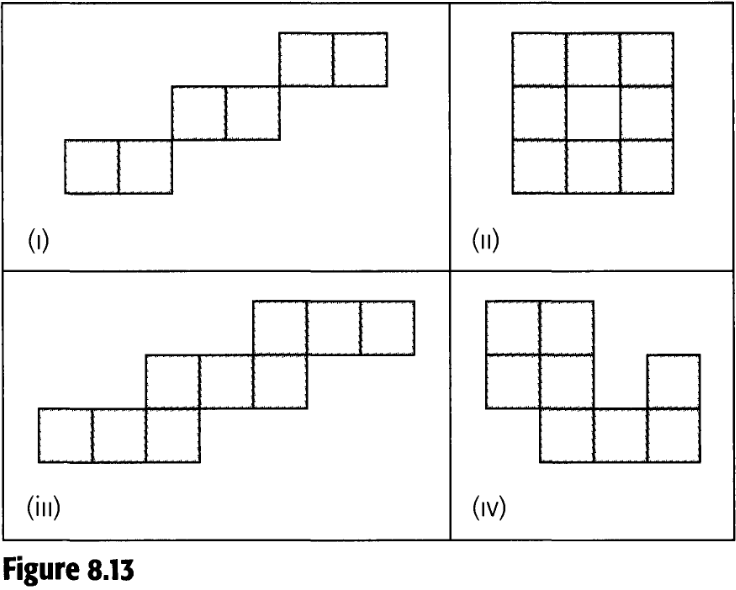
\includegraphics[scale=.4]{Photos/813.png}
		\end{center}
		
		
		\textbf{Solution:}
		
		\begin{enumerate}[label=(\alph*)]
			\item There are 4 different polynomials we have to look at, so lets look at those:
				\begin{enumerate}[label=(\roman*)]
					\item If we do rook polynomials you'll find that for $r_1$ the possible positions (being numbered
						from boxes left to right) are the amount of boxes we have available to us, being 6. After this is $r_2$
						 which would be all the possible 2 rooks we could place in this board. This would the cardinality of the
						 set: \{[1,3], [1,4], [1,5], [1,6], [2,3], [2,4], [2,5], [2,6], [3,5], [3,6], [4,5], 4,6\}. Lastly is all
						 the possible 3 rooks we could place on the board in $r_3$. This would be the cardinality of the set:
						 \{[1,3,5], [1,3,6], [1,4,5], [1,4,6], [2,3,5], [2,3,6], [2,4,5], [2,4,6]\} and would then result in the
						 equation:
						\begin{align*}
							\mathbf{1+6x+12x^2+8x^3}
						\end{align*}
					\item Let's label each of the boxes in this chessboard from top right as 1 and follow right as 2,3. Underneath
						the first row would be 4,5,6, and underneath that would be 7,8,9. To start off $r_1$ is equal to the 
						amount of blocks we have available to us which would be 9. Now for $r_2$, which would be the cardinality
						of the set: \{[1,5], [1,6], [1,8], [1,9], [2,4], [2,6], [2,7], [2,9], [3,4], [3,5], [3,8], [3,9], 
						[4,8], [4,9], [5,7], [5,9], [6,7], [6,9]\} which would be 18. For $r_3$ it is the cardinality of the set
						\{[1,5,9], [1,6,8], [2,4,9], [2,6,7], [3,5,7], [3,4,8]\} which is 6. $r_4$ doesn't exist, so this then
						ends our rook polynomial, which leads to the equation:
						\begin{align*}
							\mathbf{1+9x+18x^2+6x^3}
						\end{align*}
					\item Lets number the third from the bottom left as 1,2,3, the row right above as 4,5,6, and the 
						last row above that as 7,8,9. To start, the $r_1$ value is the amount of 9. The $r_2$, is 
						is the cardinality of the set: \{[1,4], [1,5], [1,6], [1,7], [1,8], [1,9], [2,4], [2,5], [2,6], [2,7],
						[2,8], [2,9], [3,5], [3,6], [3,7], [3,8], [3,9], [4,7], [4,8], [4,9], [5,7], [5,8], [5,9], [6,8], [6,9]\}.
						Last is to find the cardinality of the set $r_3$ which is the items \{[1,4,7], [1,4,8], [1,4,9], 
						[1,5,7], [1,5,8], [1,5,9], [1,6,8], [1,6,9], [2,4,7], [2,4,8], [2,4,9], [2,5,7], [2,5,8], [2,5,9],
						[2,6,8], [2,6,9], [3,5,7], [3,5,8], [3,5,9], [3,6,8], [3,6,9]\} which is 20 items.
						This would result in the equation:
						\begin{align*}
							\mathbf{1+9x+25x^2+20x^3}
						\end{align*}
					\item from left to right, starting at the top row, we will number the blocks. The top row is 1,2,the row below
						3,4,5, and the last row below that is 6,7,8. To start, $r_1$ is 8. $r_2$ is the cardinality of the set:
						\{[1,4], [1,5], [1,6], [1,7], [1,8], [2,3], [2,5], [2,7], [2,8], [3,6], [3,7], [3,8], [4,7], [4,8]
						[5,6], [5,7]\} which is 15. The set $r_3$ is \{[1,4,7], [1,4,8], [1,5,6], [1,5,7], [2,3,7] ,[2,3,8]
						[2,5,7], [2,5,8]\}, and it has a cardinality of 8. 
						\begin{align*}
							\mathbf{1+8x+15x^2+8x^3}
						\end{align*}
				\end{enumerate}
			
			\item I think the easiest generalization for 8.13(i) is $\mathbf{(1+2x)^3}$
			
		\end{enumerate}		
	\end{homeworkProblem} 

	%%%%%%%%%%%%%%%%%%%%%%%%%%%%%%%%%%%%%%%%%%%%%%%%%%%%%%%%%%%%%%%%%%%%%%%%%%%%%%%%%%
	%                                                                                %
	%                       Section 8.4 & 8.5 Problem 7                              %
	%                                                                                %
	%%%%%%%%%%%%%%%%%%%%%%%%%%%%%%%%%%%%%%%%%%%%%%%%%%%%%%%%%%%%%%%%%%%%%%%%%%%%%%%%%%
	
	\begin{homeworkProblem}[Problem 7]
		\tab Professor Ruth has five graders to correct programs in her courses in Java, C++, SQL, 
		Perl, and VHDL. Graders Jeanne and Charles both dislike SQL, Sandra wants to avoid C++ and VHDL.
		Paul detests Java and C++, and Todd refuses to work in SQL and Perl. In how many ways can Professor
		Ruth assign each grader to correct programs in one language, cover all five languages, and keep
		everyone content?
		
		
		\textbf{\\Solution:\\}
		
		\tab If we start by noting all 5 langauges \{Java, C++, SQL, Perl, VHDL\}, and think of this as the
		columns of our chessboard and the 5 people \{Jeanne, Charles, Sandra, Paul, Todd\} as the rows of
		our chessboard, we will get a board that looks like:
		\begin{center}
			\begin{tabular}{|c|c|c|c|c|}
				\hline
				&  & \cellcolor{black!55}X&  &   \\
				\hline
				& &\cellcolor{black!55}X &  &   \\
				\hline
				& \cellcolor{black!55}X& &  & \cellcolor{black!55}X  \\
				\hline 
				\cellcolor{black!55}X& \cellcolor{black!55}X& &  &   \\
				\hline
				& &\cellcolor{black!55}X &\cellcolor{black!55}X  &   \\
				\hline
			\end{tabular}
		\end{center}
	
		\tab We can use the rook polynomials on this. Lets start with the shaded blocks at the top as 1, row below is 2,
		the row below, from left to right, is 3,4, the row below that is 5,6, and the row below that is 7,8. For the $r_1$ value
		it would be 8. The $r_2$ value would be: \{[1,3], [1,4], [1,5], [1,6], [1,8], [2,3], [2,4], [2,5], [2,6], [2,8], 
		[3,5], [3,7], [3,8], [4,5], [4,6], [4,7], [4,8], [5,7], [5,8], [6,7], [6,8]\} and the cardinality is 21. For $r_3$ 
		it is \{[1,3,5], [1,3,7], [1,3,8], [1,4,5], [1,4,6], [1,4,7], [1,4,8], [2,3,5], [2,3,7], [2,3,8], [2,4,5], [2,4,6],
		[2,4,7], [2,4,8], [3,5,7], [3,5,8], [4,5,7], [4,5,8], [4,6,7], [4,6,8],\} which has a cardinality of 20. Next is $r_4$
		which has the set: \{[1,3,5,8], [1,4,5,8], [1,4,6,8], [2,3,5,8], [2,4,5,8], [2,4,6,8]\} which has a cardinality of 6. With
		This we can get the equation:
		\begin{align*}
			1+8x+21x^2+20x^3+12x^4
		\end{align*}
		\tab Now, from here we have to understand that we have 5 languages that we are working with and need to use the rules of
		inclusion and exclusion in order to get a concrete answer. So we can replace x with the proper value that would be in its
		place (ex. N would be 5! N($c_1$) would be 4!, etc, for the use of each language.). This would make the equation:
		\begin{align*}
			5!-(8\times 4!)+(21\times 3!)-(20\times 2!)+6=\mathbf{20}
		\end{align*}
	\end{homeworkProblem} 

	%%%%%%%%%%%%%%%%%%%%%%%%%%%%%%%%%%%%%%%%%%%%%%%%%%%%%%%%%%%%%%%%%%%%%%%%%%%%%%%%%%
	%                                                                                %
	%                       Section 8.4 & 8.5 Problem 11                             %
	%                                                                                %
	%%%%%%%%%%%%%%%%%%%%%%%%%%%%%%%%%%%%%%%%%%%%%%%%%%%%%%%%%%%%%%%%%%%%%%%%%%%%%%%%%%
	
	\begin{homeworkProblem}[Problem 11]
		\tab A computer dating service wants to match each of four women with one of six men. According to the information these
		applicants provided when they joined the service, we can draw the following conclusions.
		\begin{itemize}
			\item Woman 1 would not be compatible with man 1, 3, or 6. 
			\item Woman 2 would not be compatible with man 2 or 4.
			\item Woman 3 would not be compatible with man 3 or 6.
			\item Woman 4 would not be compatible with man 4 or 5.
		\end{itemize}
		\tab In how many ways can the service successfully match each of the four women with a compatible partner?
		
		
		\textbf{\\Solution:\\} 
		\tab So immediately, I want to create a chessboard style table to describe this. The columns are the men
		ordered 1-6 and the rows are women ordered 1-4. 
		\begin{center}
			\begin{tabular}{|l|l|l|l|l|l|}
				\hline
				 \cellcolor{black!55}X&  &\cellcolor{black!55}X&  &  &\cellcolor{black!55}X  \\
				 \hline
				 &  \cellcolor{black!55}X&  & \cellcolor{black!55}X &  &  \\
				 \hline
				 &  &  \cellcolor{black!55}X&  &  &\cellcolor{black!55}X  \\
				 \hline
				 &  &  &  \cellcolor{black!55}X& \cellcolor{black!55}X &  \\
				 \hline
			\end{tabular}
		\end{center}
		
		\tab from left to right, top to bottom, lets organize the blocks to numbers. The top rows blocks will be 1,2,3, the next
		row will be 4,5, the row after will be 6,7, the row after will be 8,9. The $r_1$ value is 9 to start off. The $r_2$ value
		is the cardinality of set \{[1,4], [1,5], [1,6], [1,7], [1,8], [1,9], [2,3], [2,4], [2,6], [2,7], [2,8], [3,4], 
		[3,5], [3,6], [3,8], [3,9], [4,6], [4,7], [4,8], [4,9], [5,6], [5,7], [5,9], [6,8], [6,9], [7,8], [7,9]\} which is
		27. The $r_3$ set is \{[1,4,6], [1,4,7], [1,4,8], [1,4,9], [1,5,6], [1,5,7], [1,5,9], [1,6,8], [1,6,9], [1,7,8], [1,7,9]
		[2,4,7], [2,4,8], [2,4,9], [2,5,7], [2,5,9], [2,7,8], [2,7,9], [3,4,6], [3,4,8], [3,4,9], [3,5,6],
		[3,5,9], [3,6,8], [3,6,9], [4,6,8], [4,6,9], [4,7,8], [4,7,9], [5,6,9], [5,7,9]\} which has a massive cardinality of 31.
		After this is $r_4$ which is the cardinality of the set \{[1,4,6,8], [1,4,6,9], [1,4,7,8], [1,4,7,9], [1,5,6,9], 
		[1,5,7,9], [2,4,7,8], [2,4,7,9], [2,5,7,9], [3,4,6,8], [3,4,6,9], [3,5,6,9], [3,5,7,9]\} which is 13. With all this I
		will get the equation:
		\begin{align*}
			1+9x+27x^2+31x^3+13x^4
		\end{align*}
		\tab Now to get the amount of ways we have to follow a similar style to what we did in Problem 7, except slightly different
		because we have a differing number of horizontal rows and vertical rows. we have to then have $N=\frac{6!}{2!}$ and
		then $\frac{5!}{2!}$ as 2 is the difference between the col and row. count down the top factorial. This would look like:
		\begin{align*}
			\frac{6!}{2!}-\left(9\times \frac{5!}{2!}\right)+\left(27\times\frac{4!}{2!}\right)-\left(31\times
			\frac{3!}{2!}\right)+\left(13\times \frac{2!}{2!}\right)=\mathbf{64}
		\end{align*}
	\end{homeworkProblem}
	
\end{document}